\hypertarget{ht__find_8c}{
\section{ht\_\-find.c File Reference}
\label{ht__find_8c}\index{ht_find.c@{ht\_\-find.c}}
}


\subsection{Detailed Description}
\begin{Desc}
\item[For internal use only.]
This file contains the implementation of the \hyperlink{group__dbprim__hash_ga13}{ht\_\-find()} function, used to locate a specific entry in a hash table.\end{Desc}


Definition in file \hyperlink{ht__find_8c-source}{ht\_\-find.c}.

{\tt \#include \char`\"{}dbprim.h\char`\"{}}\par
{\tt \#include \char`\"{}dbprim\_\-int.h\char`\"{}}\par


Include dependency graph for ht\_\-find.c:\begin{figure}[H]
\begin{center}
\leavevmode
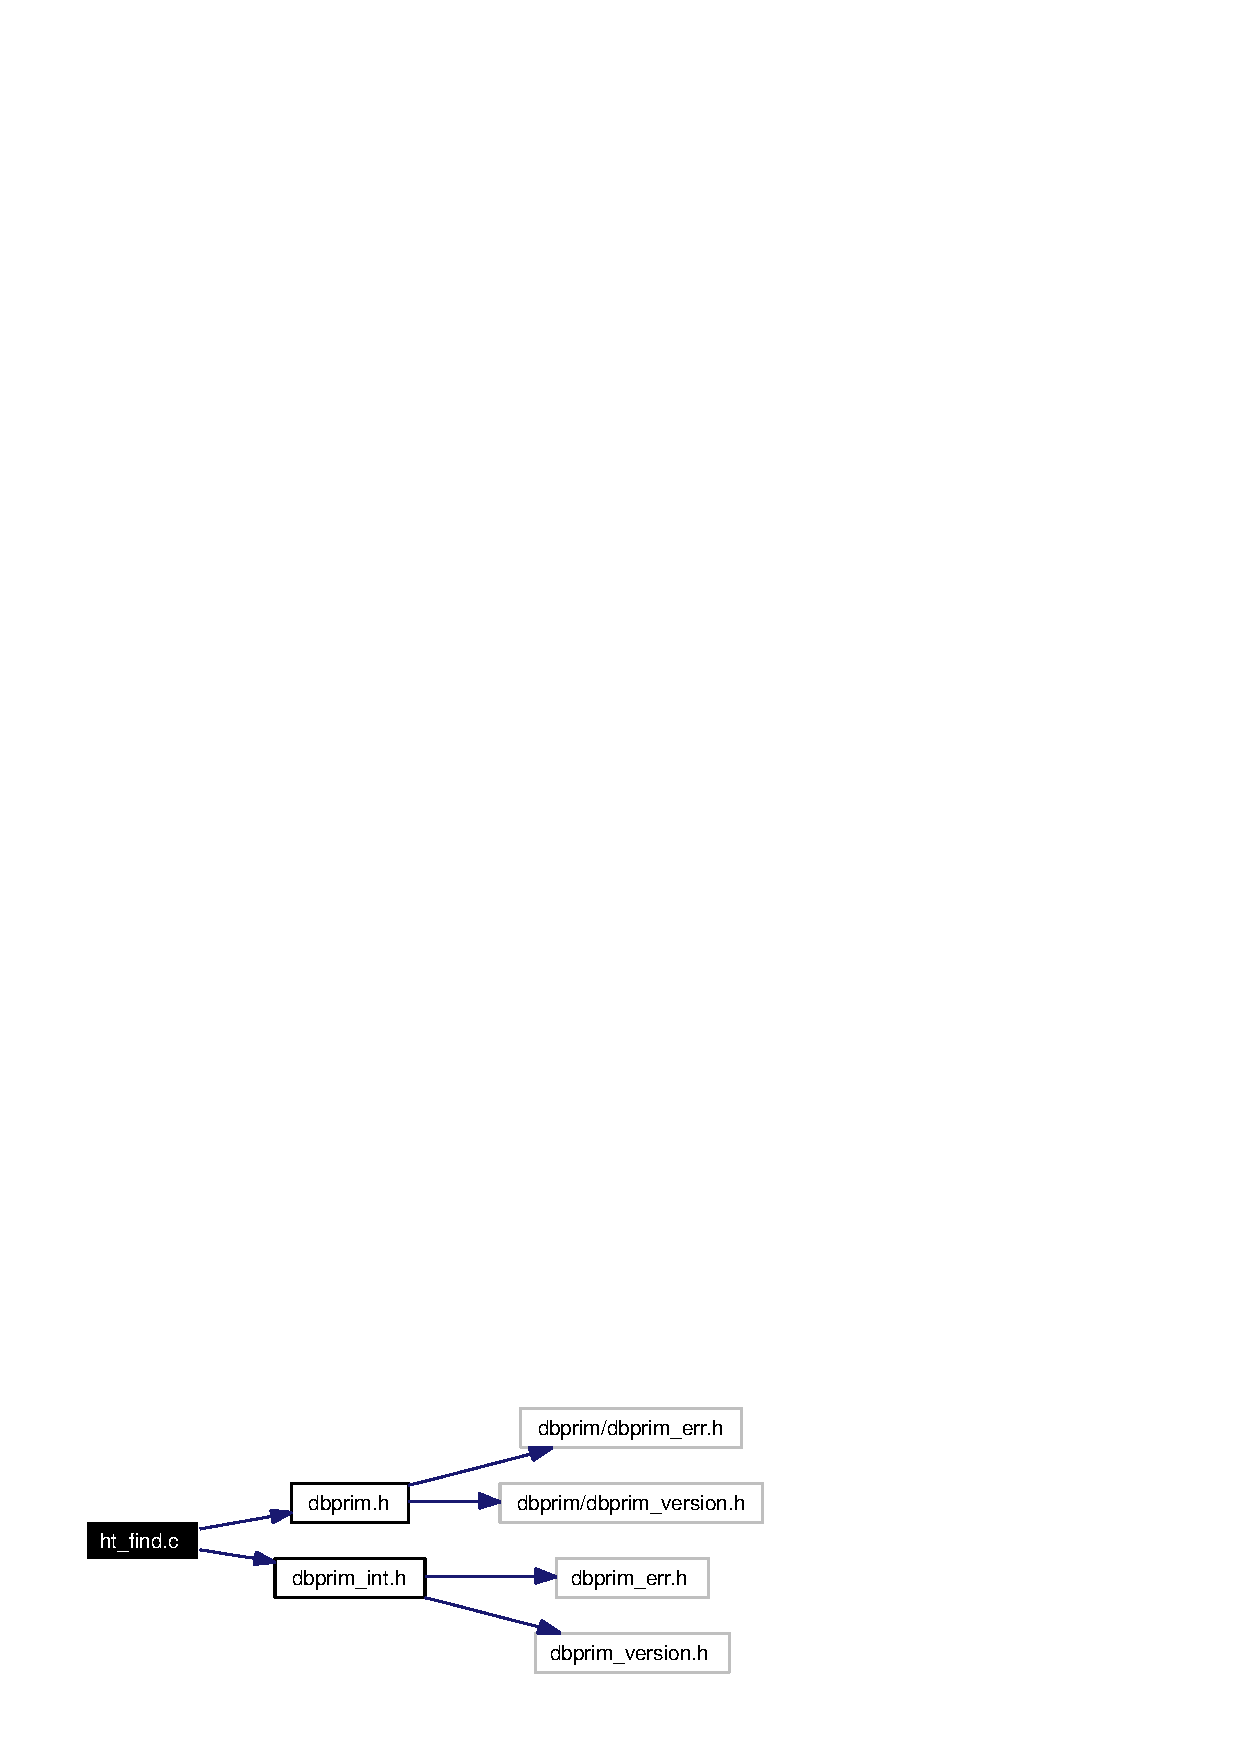
\includegraphics[width=185pt]{ht__find_8c__incl}
\end{center}
\end{figure}
\subsection*{Functions}
\begin{CompactItemize}
\item 
unsigned long \hyperlink{group__dbprim__hash_ga13}{ht\_\-find} (\hyperlink{struct__hash__table__s}{hash\_\-table\_\-t} $\ast$table, \hyperlink{struct__hash__entry__s}{hash\_\-entry\_\-t} $\ast$$\ast$entry\_\-p, \hyperlink{struct__db__key__s}{db\_\-key\_\-t} $\ast$key)
\begin{CompactList}\small\item\em Find an entry in a hash table. \item\end{CompactList}\end{CompactItemize}
